\chapter{}
Entre cinco e seis anos, contraí uma infecção séria. Ao calçar-me os sapatos novos de ir à missa, minha mãe não conseguiu afivelá-los. 
Meus pés estavam estufados como bolos. 
Chamou papai e a fisionomia assustada de ambos me causou estranheza, já que eu não estava sentindo absolutamente nada. 
Mas logo comecei a gostar dos movimentos que se seguiram porque percebi que eu me tornava o centro de alguma coisa muito importante. 
Um médico foi chamado, o que de si já era incomum, pois todas as nossas indisposições eram ordinariamente atendidas pelo Joãozinho da Farmácia.
E quando o Dr. Newton, após examinar-me, ordenou repouso absoluto e dieta, a preocupação que se estampou na face dos meus pais me convenceu em definitivo de que naquele momento, nada mais importava na face da terra senão eu.  
Olhando em retrospectiva aquele momento e os meses que se seguiram àquela manhã, espanto-me com a descoberta de quanto senso dramático pode uma criança extrair de si e que insuspeitado talento ela pode manifestar em usá-lo. 
 
Embora a situação toda me fascinasse pelo muito de atenção que atraía sobre a minha pequena pessoa, a verdade é que o processo caminhou para uma quase tragédia. 
O tal médico, Dr. Newton, cometeu um equívoco no diagnóstico inicial e o que era uma simples infecção urinária evoluiu para uma nefrite. 
Dois meses depois, o crescente entra-e-sai de parentes e vizinhos no meu quarto atestava a gravidade progressiva do quadro. Exclamações como ``pobrezinha'', ``coitadinha'' e até ``santinha'', entreouvidas entre sussurros, tornaram mais doce o sorriso que eu abria para as pessoas. 
Vovó Didi ensinou-me uma cançoneta napolitana que falava em despedida e que com voz não menos doce eu cantava para as visitas, maravilhada em ver brotar-lhes lágrimas nos olhos. 
Eu continuava a não sentir nada, de modo que podia dedicar-me integralmente a desfrutar toda a intensidade das emoções que observava ao meu redor. 
Até que um dia, no final da tarde, um pequeno tumulto formou-se na sala em torno do meu pai que acabara de chegar da rua e entre gritos e choro sentido ameaçava matar o médico. 
Eu tinha sido desenganada. 
Nenhum outro médico aceitara levar adiante meu caso e todos haviam aconselhado vivamente a família a procurar com urgência um centro maior, com mais recursos.  Naquela mesma noite, numa tumultuada partida, embarcamos no trem noturno para São Paulo e de lá, de avião, para o Rio de Janeiro, onde nos aguardavam os dois irmãos médicos do papai, Tio Zico e Tio Ângelo. 
Quando finalmente meu pai pode me descer do colo ao chão no consultório do célebre nefrologista Prof. Laclette, um engraçado velhinho com jeito de Papai Noel, amontoei diante dele como um saco de batatas. 
Meus ossos haviam se transformado em gelatina durante o prolongado repouso. 

Ficamos por quase dois meses hospedados no Engenho Velho, na casa do Tio Ângelo. 
Era preciso primeiro vencer a infecção para que o foco de todo o mal que me afetara pudesse ser extirpado: eu tinha que retirar as amídalas. 

Meu anfitrião era casado com uma exótica e linda potiguar, tia Mariazinha, que, entre outras extravagâncias, era mãe-de-santo e dona de um terreiro de umbanda. 
Era, além disso, fantástica florista, chapeleira renomada e tinha, entre os animais domésticos, um grande e assustador cachorro preto, um mico endiabrado e uma jiboia obesa. 
Tudo isso somado tornava aquela casa meio mágica para mim, sensação que minha mãe estava longe de partilhar. 
As esquisitices da Tia Mariazinha pareciam demasiadas para ela. 
Principalmente quando, logo de manhã, a cunhada vinha lhe dar bom dia trazendo enrodilhada ao pescoço, como uma estola, a enorme cobra. Ou quando mamãe se punha a dedilhar o lindo piano alemão da sala e o mico, encarapitado no lustre, saltava-lhe diretamente nos ombros. 
Era louco por música, diziam.

\begin{figure}[H]
\centering
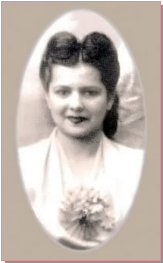
\includegraphics[width = 0.4\linewidth]{4/Tia Mariazinha.png}
\caption{A bela Tia Mariazinha.}
\end{figure}

Um acordo firmado entre marido e mulher vetava a realização de sessões de umbanda na casa. 
Para isso, Tio Ângelo havia concordado com a construção do terreiro, ou do Centro, como a Tia Mariazinha o chamava, num outro local. 
Entretanto, minha doença, ao que parece, forneceu à espevitada mãe-de-santo uma excelente oportunidade de provar a superioridade do poder dos orixás sobre a vã medicina dos civilizados. 
Logo ao chegar, eu tinha sido besuntada com óleos perfumados e metida num camisolão de flanela vermelha para desencorajar os maus espíritos. 
Em seguida, fui engalanada com voltas e voltas de guias de santo coloridas em torno do pescoço. 
Durante todo tempo em que lá estive até receber alta, foi vestida nessa flamejante indumentária que percorri consultórios e hospitais. 
Meus pais ficavam embaraçadíssimos, mas eu me achava linda. 

Como meu tio frequentemente passava noites de plantão na sua casa de saúde em Madureira, minha tia sentiu-se encorajada a ignorar o protocolo firmado com o marido e convocou seu pessoal para uma sessão noturna das importantes ali mesmo, no sagrado recinto do seu lar, já que eu, a paciente, não podia abandonar o repouso para ir ao terreiro. 
E foi desse modo que uma noite, no meio do sono, fui desperta para viver uma experiência inesquecível: no quarto semi-iluminado por velas, uma porção de gente vestida de branco entrava para dançar e cantar ao redor da minha cama, ao som do batuque ritmado dos atabaques. 
Mas o espetáculo maior era ela, minha tia: à frente de todos, numa roupa de alvura deslumbrante, enfeitada de colares, pulseiras e balangandãs, babados e mais babados de renda flutuando em imensa nuvem em torno do corpo, ela girava e sambava soberana, esplêndida Iemanjá! 
Pela primeira vez, vi os cabelos que ela arrumava em grosso rolo sobre a nuca, derramados em cascata negra e brilhante até abaixo da cintura. 
Sobre a cabeça, em equilíbrio milagrosamente inalterado pelos passos da dança, um copo de cristal com conchas e água do mar.
 Nunca mais me passou a vontade de um dia me vestir daquela maneira e dançar como a vi fazer naquela noite, deusa branca do candomblé. 
Dias depois, Tia Mariazinha achou necessário fazer uma nova sessão para reforçar os efeitos da primeira. 
Não vi o que aconteceu. 
A casa era um sobrado sólido, de grossas paredes, e eu já adormecera no andar de cima. 
Mas mamãe contou que meu tio chegou inesperadamente e o ritual foi abortado pela mais fulgurante explosão de ira que ela já tinha presenciado num Filpi. 
Caboclos, exus, babalaôs e babalorixás desceram desabalados rua abaixo. Não sobrou um para contar história. 

Ao fim de três semanas, já operada da garganta, comecei a melhorar e assim que me libertei do repouso, passei a freqüentar a oficina do quintal, onde a tia fazia inacreditáveis e delicadas camélias de veludo e cetim, rosas e violetas de organdi e seda e as arrumava em elegantes arranjos que as senhoras usavam à lapela dos ``tailleurs'', no decote, à cintura dos vestidos ``soirée'', ou ainda sobre a aba dos lindos chapéus que saíam daqueles dedos habilidosos e iam sendo arrumados em caixas sobre um tabuleiro enorme que depois ela punha à cabeça e, com seu displicente gingado de cabrocha, ia entregar nas casas das freguesas.

No aniversário da minha mãe, essa nordestina que jamais usou seu sofisticado bom gosto em favor de si mesma, orientou meu pai a comprar um corte de organza e renda francesas na ``Casa Canadá'', templo da moda carioca de então. 
Dentro da embalagem, sobre o negro transparente dos preciosos tecidos, colocou um ramo de rosas de organdi. 
Nunca vi outro igual. 
Foi o traje mais aristocrático que a minha mãe teve em toda sua vida. 

Uma semana depois, liberada já pelos médicos, preparava\hyp{}me para voltar para casa. Não sem antes conhecer o mar, o Corcovado, subir de bondinho o Pão de Açúcar e tomar sorvete na Confeitaria Colombo. 
Tinha viajado de trem e, suprema ventura, pela segunda vez ia tomar um avião. 
Na vinda tinha sido um Viscount e na volta seria um Constellation. 

Antes de partirmos, Tia Mariazinha exigiu que meu pai enchesse de moedas uma gamela de barro para ser enterrada lá em cima do morro, em sinal de gratidão às entidades às quais, na opinião dela, eu incontestavelmente devia minha cura. 
Por via das dúvidas, ele achou prudente não contrariar. 
E lá foi ela, encosta acima, gamela equilibrada sobre a cabeça, confiante para todo o sempre no poder e na proteção das suas bárbaras divindades. 
Por causa desta fé, quando, muitos anos depois da morte do meu tio, bastante doente e sofrendo dores terríveis, ela permitiu que seu filho finalmente a entregasse aos médicos, já era tarde: um câncer devastador tomara conta do seu corpo e nada mais havia para fazer. 

Ainda hoje são vívidos na minha lembrança a preocupação, a atenção e o carinho beirando a ternura com que os meus tios Ângelo, Zico, Bepe e, principalmente, meu próprio pai, que tinham como denominador comum o gênio tempestuoso e o pavio demasiadamente curto, cuidaram de mim e mantiveram em suspenso suas próprias vidas até me ver restabelecida. 
Como também nunca esqueci as noites em claro da minha mãe à minha cabeceira e seus cuidados incessantes, exclusivos e quase ciumentos, capítulos de um longo aprendizado do exercício da maternidade que ela então começou a me ensinar.

De todo o episódio, restou-me a descoberta de uma veia dramática que eu continuaria a explorar em favor dos meus objetivos, sem nenhum pudor, e um campo maior e mais rico para os meus devaneios de menina.
Eu tinha descoberto um mundo para além das ruas da minha cidade. 
Comecei a me interessar por moda e desenhava mocinhas copiadas das revistas ostentando flores no cabelo, nos vestidos esvoaçantes e nos chapéus.  
E acho que me ficou, lá no fundo, fruto da convivência com a estranha tia macumbeira, sua cobra e seu animismo, uma empatia em estado de dormência que haveria de se manifestar no dia em que, através da leitura de Gabriel Garcia Márquez, fui apresentada ao estilo, às histórias e personagens delirantes dos escritores do realismo mágico latino-americano.

Na fase araraquarense da doença, o sacrifício imposto pelo longo período de repouso atenuou-o a alegre e redonda Ondina, empregada da fábrica do meu pai, que todos chamavam pelo curto e marinho apelido de Onda e que, posta a zelar diariamente para que eu não me agitasse, ensinou-me a fazer roupinhas de boneca. 
Caiu-me tanto no gosto a brincadeira que ainda as fazia, já mulher feita, para vestir as bonecas da Paula.

Acho que se acirrou, também, a partir daí, uma longa relação de rivalidades e atritos que marcaria, por muitos e muitos anos, a convivência entre mim e Reginaldo, meu irmão mais próximo. 
Por cerca de seis meses a família gravitara quase exclusivamente em torno da minha saúde. 
A partida para o Rio de Janeiro fora abrupta e ele, com quatro anos, tinha sido deixado sem maiores explicações aos cuidados do Tio Totó, o irmão do meu pai que morava na fazenda e que, entre todos os Filpi, era o mais rude e severo. Se tivesse nascido nos dias de hoje, creio, meu irmão seria diagnosticado como uma criança hiperativa. 
Era magricela, agitado e provocador. 
Com certeza foi submetido, mais de uma vez, aos duros métodos do Tio Totó. 
O fato é que quando, ao voltar, meus pais foram buscá-lo na fazenda, tiveram que caçá-lo no meio do pasto como a um potro bagual. 
Ele corria e gritava que não era filho deles. 
Até a idade adulta, vez ou outra, entre brincando e sério, ele manteve o estranho hábito de perguntar à minha mãe se não era verdade que fora adotado. 
E, por igual período, pareceu sentir enorme prazer em me atazanar sempre que a ocasião se apresentasse propícia. 

Para finalizar, minha mãe ficou presa de uma ansiedade que ela só conseguia resolver ministrando-me quantidades enormes de mingau de aveia e certificando-se, refeição após refeição, de que eu não deixara sobrar nada no prato. Quatro anos depois, eu me tornara uma criança obesa.
